\documentclass[11pt]{article}
\usepackage[a4paper,margin=1in]{geometry}
\usepackage[T1]{fontenc}
\usepackage{lmodern}
\usepackage{amsmath,amssymb,amsthm}
\usepackage{booktabs}
\usepackage{graphicx}
\usepackage{xcolor}
\usepackage[numbers,sort&compress]{natbib}
\usepackage[colorlinks=true,linkcolor=blue!50!black,citecolor=blue!50!black,urlcolor=blue!50!black]{hyperref}
\usepackage{enumitem}
\setlist{nosep,leftmargin=*}
\newtheorem{proposition}{Proposition}
\newtheorem{definition}{Definition}
\newcommand{\AtlasArch}{0.081}
\newcommand{\AtlasFamily}{0.045}
\newcommand{\AtlasGraphArch}{1.20}
\newcommand{\AtlasGraphFamily}{1.49}
\newcommand{\AtlasGraphModel}{1.51}
\newcommand{\AtlasModel}{0.301}
\newcommand{\AtlasNArch}{20}
\newcommand{\AtlasNFamily}{12}
\newcommand{\AtlasNModel}{8}
\newcommand{\AtlasPredArch}{1.10}
\newcommand{\AtlasPredFamily}{1.06}
\newcommand{\AtlasPredModel}{1.47}
\newcommand{\CovCovFive}{0.920}
\newcommand{\CovCovFour}{0.948}
\newcommand{\CovCovSix}{0.960}
\newcommand{\CovCovThree}{0.946}
\newcommand{\CovCovTwo}{0.909}
\newcommand{\CovGregFive}{0.950}
\newcommand{\CovGregFour}{0.907}
\newcommand{\CovGregMinFive}{0.812}
\newcommand{\CovGregMinFour}{0.625}
\newcommand{\CovGregMinSix}{0.895}
\newcommand{\CovGregSix}{0.944}
\newcommand{\CovMinGraphTwo}{0.677}
\newcommand{\CovRstratFive}{0.984}
\newcommand{\CovRstratFour}{0.985}
\newcommand{\CovRstratSix}{0.988}
\newcommand{\DecGraphFive}{3.9}
\newcommand{\DecGraphFour}{6.5}
\newcommand{\DecGraphSix}{6.0}
\newcommand{\DecGregAllFive}{24.0}
\newcommand{\DecGregExtFive}{87}
\newcommand{\DecGregFive}{9.3}
\newcommand{\DecGregFour}{8.4}
\newcommand{\DecGregSix}{4.3}
\newcommand{\DecNFive}{12}
\newcommand{\DecNFour}{21}
\newcommand{\DecNSix}{17}
\newcommand{\DecRedFive}{49}
\newcommand{\DecRedFour}{54}
\newcommand{\DecRedSix}{32}
\newcommand{\DecResetAllFive}{13.0}
\newcommand{\DecResetExtFive}{0}
\newcommand{\DecResetFive}{7.6}
\newcommand{\DecResetFour}{14.1}
\newcommand{\DecResetSix}{8.8}
\newcommand{\DecRstratFive}{5.0}
\newcommand{\DecRstratFour}{7.2}
\newcommand{\DecRstratSix}{4.1}
\newcommand{\DemoCov}{100}
\newcommand{\DemoGood}{78}
\newcommand{\DetFA}{0.8}
\newcommand{\DetN}{11}
\newcommand{\DetNok}{73}
\newcommand{\DetPower}{92}
\newcommand{\DetProbes}{30}
\newcommand{\EquivProbesFive}{32}
\newcommand{\EquivProbesFour}{43}
\newcommand{\EquivProbesSix}{44}
\newcommand{\EquivProbesSixStrat}{45}
\newcommand{\EtaMedFive}{0.35}
\newcommand{\EtaMedFour}{0.54}
\newcommand{\EtaMedSix}{0.57}
\newcommand{\FiveLowN}{21}
\newcommand{\GCfSeven}{1.955}
\newcommand{\GEcoOnlyThree}{2.006}
\newcommand{\GGraphFive}{1.12}
\newcommand{\GGraphFour}{1.95}
\newcommand{\GGraphMinFive}{0.71}
\newcommand{\GGraphMinFour}{0.76}
\newcommand{\GGraphMinSix}{1.15}
\newcommand{\GGraphMinThree}{0.60}
\newcommand{\GGraphMinTwo}{0.38}
\newcommand{\GGraphSix}{1.77}
\newcommand{\GGraphThree}{2.01}
\newcommand{\GGraphThreePrecise}{2.014}
\newcommand{\GGraphTwo}{1.39}
\newcommand{\GGregFive}{1.61}
\newcommand{\GGregFiveLow}{1.51}
\newcommand{\GGregFour}{1.84}
\newcommand{\GGregMinFive}{1.08}
\newcommand{\GGregMinFour}{1.06}
\newcommand{\GGregMinSix}{1.45}
\newcommand{\GGregSix}{2.20}
\newcommand{\GKnnSeven}{1.937}
\newcommand{\GPredFive}{1.22}
\newcommand{\GPredFour}{1.47}
\newcommand{\GPredMinFive}{0.88}
\newcommand{\GPredMinFour}{0.93}
\newcommand{\GPredMinSix}{0.97}
\newcommand{\GPredMinThree}{0.61}
\newcommand{\GPredMinTwo}{0.75}
\newcommand{\GPredPilot}{1.22}
\newcommand{\GPredSix}{1.56}
\newcommand{\GPredThree}{1.53}
\newcommand{\GPredTwo}{1.12}
\newcommand{\GRstratFive}{1.27}
\newcommand{\GRstratFour}{1.93}
\newcommand{\GRstratMinFive}{0.73}
\newcommand{\GRstratMinFour}{1.09}
\newcommand{\GRstratMinSix}{1.34}
\newcommand{\GRstratMinXFive}{0.73}
\newcommand{\GRstratMinXFour}{1.09}
\newcommand{\GRstratMinXSix}{1.34}
\newcommand{\GRstratSix}{2.12}
\newcommand{\GStratFive}{1.21}
\newcommand{\GStratFiveHigh}{1.94}
\newcommand{\GStratFour}{2.14}
\newcommand{\GStratMinFive}{0.58}
\newcommand{\GStratMinFiveLow}{0.58}
\newcommand{\GStratMinFour}{0.91}
\newcommand{\GStratMinSix}{1.17}
\newcommand{\GStratSix}{2.25}
\newcommand{\HFourTwoPower}{86}
\newcommand{\HFourTwoProbes}{52}
\newcommand{\HypFailed}{5}
\newcommand{\HypSupported}{29}
\newcommand{\HypTotal}{34}
\newcommand{\KernelCov}{0.943}
\newcommand{\KernelDec}{6.0}
\newcommand{\KernelDecReset}{11.9}
\newcommand{\KernelGain}{2.18}
\newcommand{\KnnPSeven}{0.654}
\newcommand{\KnnRatioSeven}{0.995}
\newcommand{\LawBiasFinite}{-1.1}
\newcommand{\LawBiasSuper}{+1.1}
\newcommand{\LawBigConst}{11.3}
\newcommand{\LawBigErr}{4.3}
\newcommand{\LawBigN}{75}
\newcommand{\LawCorrLog}{0.975}
\newcommand{\LawErrFinite}{4.2}
\newcommand{\LawErrFive}{5.8}
\newcommand{\LawErrFour}{3.9}
\newcommand{\LawErrPilot}{2.6}
\newcommand{\LawErrPilotProbe}{4.4}
\newcommand{\LawErrPooled}{3.9}
\newcommand{\LawErrSix}{6.4}
\newcommand{\LawErrThree}{3.6}
\newcommand{\LawErrTwo}{2.7}
\newcommand{\LawTrivShare}{20}
\newcommand{\LawWithinTen}{84}
\newcommand{\MCErr}{3}
\newcommand{\NAll}{249}
\newcommand{\NConf}{219}
\newcommand{\NFive}{33}
\newcommand{\NFour}{28}
\newcommand{\NSeven}{90}
\newcommand{\NSix}{29}
\newcommand{\NThree}{89}
\newcommand{\NTwo}{40}
\newcommand{\PGregVsRstratFive}{1.4\times10^{-5}}
\newcommand{\PGregVsRstratFour}{0.895}
\newcommand{\PGregVsRstratSix}{0.268}
\newcommand{\PStratVsRstratFive}{0.817}
\newcommand{\PStratVsRstratFour}{9.7\times10^{-5}}
\newcommand{\PStratVsRstratSix}{0.254}
\newcommand{\PhiCtrlThree}{0.316}
\newcommand{\PhiLineThree}{0.367}
\newcommand{\PilotCovBMA}{0.926}
\newcommand{\PilotN}{30}
\newcommand{\PvalFiveVsPredThree}{7.8\times10^{-14}}
\newcommand{\PvalHSevenThree}{0.038}
\newcommand{\SModelMed}{+0.033}
\newcommand{\SPermSig}{6}
\newcommand{\SProvGap}{+0.047}
\newcommand{\SProvP}{5.0\times10^{-4}}
\newcommand{\SScaffMed}{+0.060}
\newcommand{\SScaffPos}{7}
\newcommand{\SScaffVsModelMed}{+0.064}
\newcommand{\SWilcoxP}{0.008}
\newcommand{\StratBigErr}{7.3}
\newcommand{\StratBigN}{64}
\newcommand{\StratCorrLog}{0.939}
\newcommand{\StratErrFive}{7.7}
\newcommand{\StratErrFour}{8.8}
\newcommand{\StratErrPooled}{7.7}
\newcommand{\StratErrSix}{7.2}
\newcommand{\StratN}{90}
\newcommand{\ThreeMidMin}{1.25}
\newcommand{\ThreeMidN}{85}
\newcommand{\WidthGreg}{0.31}
\newcommand{\WidthReset}{0.31}
\newcommand{\WidthStrat}{0.24}
\newcommand{\WidthStratRed}{22}
\newcommand{\WorstVThree}{0.60}

\newcommand{\phisq}{\varphi^2}

\title{How Much Is an Agent's History Worth?\\[2pt]
\large A Law of Evaluation Transfer Across Agent Versions,\\ Tested in Six Pre-Registered Studies}
\author{Rayen Zargui\\
Institut Polytechnique de Paris\\
\texttt{rayen.zargui@polytechnique.edu}}
\date{November 2026}

\begin{document}
\maketitle

\begin{abstract}
Every new version of an AI agent---a new model, prompt, or scaffold---is evaluated as if nothing had been
learned before, although the outcomes of every earlier agent on the same tasks are already known. We organise
this history as a \emph{graph of agents}: nodes are agent versions, lineage edges link a version to its
predecessor, and every node carries its outcome on each task of a shared suite. We ask how many tasks that
history is worth, and answer with a closed-form law: testing $m$ tasks of a new version with the help of the
graph is as precise as testing $m/(1-\rho^2)$ tasks at random, where $\rho^2$ is the share of the new version's
task-level variance already explained by the graph---$\phisq$ with the predecessor (double sampling), $\eta^2$
with the task difficulty seen by all earlier agents (stratified sampling). We turn the law into a three-move
method: the graph \emph{chooses} the tasks, a cross-fitted model-assisted estimator \emph{estimates} the new
version's success rate with calibrated intervals, and the same tasks \emph{decide} whether to keep or replace the
current version. Every confirmatory hypothesis was pre-registered and frozen by a git tag before the data were
examined. After a
pilot on model versions, five confirmations cover \NConf{} real version transitions never analysed before:
agents on AppWorld, SWE-bench (Verified, Lite, test, multilingual), Multi-SWE-bench in seven languages, model
versions on LiveCodeBench, and office agents on TheAgentCompany. Given $\rho^2$, the law predicts the observed
efficiency gain within \LawErrPooled\% (median) across all \NConf{} transitions---the order of the simulation noise---and
within 10\% for \LawWithinTen\% of them. Most of the gain comes from letting the graph choose the tasks: with 20
graph-chosen tasks, estimates are as precise as with about \EquivProbesSix{} random tasks. The cross-fitted estimator
never lost to random testing in the last two confirmations (worst case $\times\GGregMinFive$ and
$\times\GGregMinSix$), including on versions that solve almost nothing, and its 90\% intervals covered the truth
\CovGregSix{} of the time; keep-or-replace decisions were wrong \DecRedSix--\DecRedFour\% less often than with
random testing. Of
\HypTotal{} pre-registered hypotheses, \HypSupported{} were supported; we report the \HypFailed{} failures in full.
We release a small kernel that implements the graph and reproduces the research results when replaying 89 real
SWE-bench transitions.
\end{abstract}

\section{Introduction}
Agents change constantly. A coding agent ships a new model in March, a new scaffold in May, a new prompt every
week. Each change raises the same question---is the new version better than the one in production?---and the
standard answer is to re-run the full evaluation suite. On agentic benchmarks this is expensive: a single
SWE-bench Verified run executes 500 repository-level tasks, each in its own container
\citep{jimenez2024swebench}, and office-automation suites run long multi-step tasks in simulated companies
\citep{xu2024theagentcompany}.

Yet a team that evaluates a new version is never starting from nothing. It knows how the previous version did on
every task, and how every other agent it ever tested did on the same tasks. This paper starts from a simple
picture of that knowledge, inspired by the idea of an LLM-maintained wiki of interlinked pages
\citep{karpathy2026wiki}: a \emph{graph of agents} in which each node is an agent version, lineage edges connect
successive versions, and each node carries its task-level results. The question we study is quantitative:

\begin{quote}\emph{When a new node arrives, how many tasks is the rest of the graph worth?}\end{quote}

\paragraph{Contributions.} This paper makes five contributions.
\begin{enumerate}
\item \textbf{A law of evaluation transfer} (Section~\ref{sec:law}). We show that classical results of survey
sampling---double sampling \citep{neyman1938,cochran1977} and stratification---give a closed-form prediction of
the efficiency gain an agent's history provides, $1/(1-\rho^2)$, with two measurable forms of $\rho^2$: the
predecessor's $\phisq$ and the graph's $\eta^2$. The law turns ``how much history is transferable'' into a single
measurable quantity, which can be estimated from the tested tasks themselves or anticipated from the type of change
(Table~\ref{tab:atlas}).
\item \textbf{A three-move method} (Section~\ref{sec:method}). The graph chooses the tasks (stratification on the
difficulty seen by earlier agents), which provides most of the gain; a cross-fitted generalised regression estimator
\citep{sarndal1992,zrnic2024cross} with effective-sample-size intervals \citep{korn1998} estimates the new version's
rate without catastrophic losses; the same tasks decide keep-or-replace and flag whether the decision is sure.
\item \textbf{A pre-registered evidence chain} (Section~\ref{sec:protocol}). Six studies---one pilot and five
confirmations on data never analysed before---each frozen by a git tag and SHA-256 hashes before the first
statistic, with every development step done on previously seen data only and every deviation logged.
\item \textbf{Results on \NConf{} real version transitions} (Section~\ref{sec:results}), including an atlas of
what survives a version change and \HypFailed{} pre-registered failures reported in full.
\item \textbf{A kernel} (Section~\ref{sec:kernel}) implementing the graph of agents---an append-only event log, a
registry of slots and versions, and the operations \texttt{record}, \texttt{plan}, \texttt{estimate},
\texttt{decide}, \texttt{lint}---validated by replaying 89 real transitions.
\end{enumerate}

\section{Setting}
\label{sec:setting}
A \emph{task suite} is a fixed set of $N$ tasks with binary outcomes (resolved or not). An \emph{agent version}
$v$ has an outcome vector $y_v\in\{0,1\}^N$ and a success rate $p_v=\frac1N\sum_j y_{vj}$. The \emph{graph}
$\mathcal G$ at time $t$ contains every version released before $t$ whose outcome vector is fully known, and a
lineage edge $v\to v'$ when $v'$ is the next version of the same product (the same agent \emph{slot}).

When a new version $v'$ arrives, its outcome vector is unknown. We test it on $m\ll N$ \emph{probe} tasks and must
(i) estimate $p_{v'}$ with an interval, and (ii) decide whether $p_{v'}\ge p_v$. The baseline is \emph{random
testing}: $m$ tasks drawn uniformly, estimated by their success rate (we use a Jeffreys-smoothed mean with
Clopper--Pearson-type intervals; with $m=20$ the smoothing lowers the mean squared error of the plain sample mean by
about 9\% for rates between 0.3 and 0.7, making the baseline slightly harder to beat, and raises it by about 10\% near
5\%). We measure every method by its \emph{gain}:
\begin{equation}
\mathrm{Gain} = \frac{\mathrm{MSE}(\text{random testing with } m \text{ tasks})}{\mathrm{MSE}(\text{method with } m \text{ tasks})},
\end{equation}
so that $m$ tasks with the method are worth $\mathrm{Gain}\times m$ random tasks. A gain below 1 is a loss.

\section{A law of evaluation transfer}
\label{sec:law}
\paragraph{The predecessor.} The predecessor $v$ has been measured on all $N$ tasks; the new version on $m$. This is
exactly Neyman's double sampling \citep{neyman1938}: a cheap auxiliary variable (here the predecessor's outcome)
observed on a large first-phase sample, the expensive variable on a subsample. Let $\varphi$ be the correlation
between $y_v$ and $y_{v'}$ over tasks (the phi coefficient of their $2\times2$ flip table).

\begin{proposition}[Predecessor law]\label{prop:phi}
Let the predecessor be known on all $N$ tasks and $m$ probes be drawn at random. To first order, the double-sampling
regression estimator has variance $S^2(1-\phisq)/m + \phisq S^2/N$ when tasks are viewed as draws from a
population of tasks \citep[ch.~12]{cochran1977}, where $S^2$ is the variance of $y_{v'}$. Its gain over random
testing is then
\begin{equation}\label{eq:law}
\mathrm{Gain}_{\varphi} = \frac{1}{1-\phisq+\phisq\, m/N}.
\end{equation}
If instead the target is the success rate on the $N$ tasks themselves (finite population), the second term vanishes and
the gain is $1/(1-\phisq)$.
\end{proposition}
The two targets differ by a factor $(1-\phisq+\phisq m/N)/(1-\phisq)$, close to 1 when $m\ll N$. We pre-registered
(\ref{eq:law}); our replays measure error against the finite-population rate, and the observed gains fall between the two
forms (median deviation \LawBiasSuper\% from (\ref{eq:law}) and \LawBiasFinite\% from $1/(1-\phisq)$). The estimator we
test is the Bayesian double-sampling estimator of Section~\ref{sec:method}, which behaves like post-stratification on the
predecessor's outcome when the link is informative. Either way, the gain depends on one number, $\phisq$: how much of the
new version's task-level behaviour its predecessor already explains. A minor model update keeps $\phisq$ high; a rewrite
of the agent's orchestration can erase it.

\paragraph{The graph.} The rest of the graph carries a different kind of information: which tasks are hard. Sort the
$N$ tasks by the difficulty seen by all earlier agents, cut them into $m$ contiguous strata of size $N_h\approx
N/m$ (sizes differ by at most one task), and test one task per stratum. Because the strata are built from the history
only, the probe outcomes weighted by $N_h/N$ are unbiased for $p_{v'}$; with equal-size strata this is the plain
probe mean.

\begin{proposition}[Graph law]\label{prop:eta}
Under this stratified design, the gain over random testing is
\begin{equation}\label{eq:strat}
\mathrm{Gain}_{\eta} = \frac{(1-m/N)\,S^2/m}{\frac{1}{m^2}\sum_h (1-1/N_h)\,S_h^2}\;\approx\;\frac{1}{1-\eta^2_{\mathcal G}},
\end{equation}
where $S_h^2$ is the variance of $y_{v'}$ within stratum $h$ and $\eta^2_{\mathcal G}$ is the share of its variance
explained by the strata \citep[ch.~5]{cochran1977}.
\end{proposition}

Both forms are instances of the same statement: \emph{the history is worth $1/(1-\rho^2)$ times the tasks}, where
$\rho^2$ is the fraction of the new version's task-level variance that the graph already explains. The individual
results are classical; what is new is the identification of an agent's version history with the first phase of a
two-phase design, the use of the graph of all earlier agents as the stratifier, and the empirical test that these
closed forms predict the actual gains of agent evaluation (Section~\ref{sec:res-law}).

\section{Method: choose, estimate, decide}
\label{sec:method}
\paragraph{Choose.} Compute, for each task, the logit of the smoothed success rate of all earlier agents in the
graph. Sort, form $m$ strata, draw one task per stratum (Proposition~\ref{prop:eta}). The selection uses the
history only, so it is ignorable for model-based inference and keeps the probe mean unbiased.

\paragraph{Graph predictions.} We fit a Bayesian logistic regression of the new version's probe outcomes on two
graph features---the ecosystem difficulty and the predecessor's outcome---with priors $N(0,2^2)$ on the intercept
and $N(0,1)$ on the slopes, averaging over the four covariate subsets with weights proportional to their marginal
likelihoods (estimated by importance sampling with a multivariate-$t$ proposal). This yields a probability
$\hat\pi_j$ for every task. The model-based estimate of $p_{v'}$ adds the observed probe outcomes to the predicted
outcomes of the $N-m$ untested tasks (finite-population prediction).

\paragraph{Estimate: cross-fitted GREG.} Model-based predictions are efficient but can be biased when the model
is wrong, which happens for versions that solve almost nothing. The generalised regression (GREG) estimator
\citep{sarndal1992} corrects the predictions with the residuals observed on the probes and is design-unbiased
whatever the model. Measuring residuals on the probes used to fit the model makes them too small and the intervals
too narrow; we therefore cross-fit \citep{zrnic2024cross}: strata are split into two interleaved folds, the model
fitted on one fold predicts the residuals of the other, and
\begin{equation}
\hat p_{v'} = \frac1N\sum_{j=1}^N \bar\pi_j \;+\; \frac1N\sum_{i\in\text{probes}} N_{h(i)}\,\bigl(y_{v'i}-\hat\pi^{(-k(i))}_i\bigr),
\end{equation}
where $\bar\pi$ averages the two fold models and $\hat\pi^{(-k)}$ is the model not fitted on fold $k$. Its variance
is estimated by pairing adjacent strata \citep[\S5A.12]{cochran1977}, floored at a quarter of the Jeffreys binomial
variance, and converted into an interval for a proportion at the effective sample size, with a degrees-of-freedom
correction and Jeffreys quantiles \citep{korn1998}; following \citet{brown2001}, the lower bound is 0 when no probe
succeeds and the upper bound 1 when all do.

\paragraph{Decide.} Keep $v$ or switch to $v'$ by the sign of $\hat p_{v'}-p_v$, using the model-based estimate on
the same graph-chosen probes; the decision is flagged as \emph{sure} when the GREG interval excludes $p_v$.

\paragraph{Detect regressions sequentially.} Probes arrive in batches of 10, up to 80; an alert is raised when the
upper 95\% bound of the predecessor-based (double-sampling) estimate falls below $p_v$, and testing stops early when
the lower bound exceeds $p_v-0.08$.

\paragraph{Predecessor-only baseline.} To isolate what the graph adds, we also report a Bayesian double-sampling
estimator that uses only the predecessor: it averages a model in which the new version ignores the predecessor and
a model with separate success rates after predecessor successes and failures, weighted by Beta-binomial marginal
likelihoods.

\section{Protocol}
\label{sec:protocol}
\paragraph{Pre-registration.} Each study was written as a protocol (hypotheses, thresholds, estimators, seeds,
data rules) and an analysis script, committed together and frozen by a git tag (\texttt{prereg-v1} to
\texttt{prereg-v6}) and SHA-256 hashes \emph{before any statistic was computed on its data}
\citep{nosek2018prereg}. Only format audits (file keys, task identifiers, submission names and dates) were
allowed before the freeze. Every method change was developed on data already analysed in an earlier study, never on
the data of the next confirmation. All deviations---including one accidental display of a single submission's
total during a format audit---are logged in the repository. Hashes were re-verified after each run.

\paragraph{Data.} Table~\ref{tab:data} lists the sources. Transitions are defined mechanically from public
submission names and dates: within a product lineage, each submission is paired with the latest strictly earlier
submission of the same lineage; the graph of a new version contains only submissions released strictly before it.
Tasks of SWE-bench test that also belong to Verified or Lite (analysed earlier) were removed before the freeze.

\begin{table}[t]
\centering\small
\caption{Pre-registered studies. ``Transitions'' are real version changes; ``Tasks'' is the task suite size.}
\label{tab:data}
\resizebox{\linewidth}{!}{\begin{tabular}{@{}llrrl@{}}
\toprule
Study & Source & Transitions & Tasks & Nodes are\\
\midrule
v1 (pilot) & Sheng \& Lu \citep{sheng2026regression} & \PilotN & 164--5{,}000 & model versions\\
v2 & AppWorld \citep{trivedi2024appworld} & \NTwo & 168 / 417 & 14 agents (4 scaffolds, 4 models)\\
v3 & SWE-bench Verified \citep{jimenez2024swebench} & \NThree & 500 & 175 public agents\\
v4 & SWE-bench Lite & \NFour & 300 & 84 public agents\\
v5 & Multi-SWE-bench \citep{zan2025multiswe} (7 lang.), & \NFive & 128--1{,}587 & public agents\\
 & SWE-bench test and multilingual & & & \\
v6 & LiveCodeBench \citep{jain2024livecodebench}, & \NSix & 713 / 175 & models; office agents\\
 & TheAgentCompany \citep{xu2024theagentcompany} & & & \\
\midrule
Total (confirmations v2--v6) & & \NConf & & \\
\bottomrule
\end{tabular}}
\end{table}

\paragraph{Replays.} For every transition we simulate the evaluation of the new version 400 times (1{,}000 in the
pilot): draw the probes (uniformly, or with the graph's stratified design, independently), apply every estimator to
the same probes, and compare with the true rate measured on all $N$ tasks. The primary budget is $m=20$; $m=40$ is
reported as secondary. Coverage is the fraction of replays whose 90\% interval contains the truth.

\section{Results}
\label{sec:results}

\subsection{The law predicts the gain}\label{sec:res-law}
Figure~\ref{fig:law} plots predicted against observed gains. The predecessor law (\ref{eq:law}), evaluated at the
true $\phisq$, predicts the gain of the double-sampling estimator within \LawErrPooled\% (median absolute relative
error) over the \NConf{} confirmation transitions; the correlation of log-gains is \LawCorrLog. The error is
\LawErrTwo\%, \LawErrThree\%, \LawErrFour\%, \LawErrFive\% and \LawErrSix\% in the five confirmations, and
\LawErrPilot\% in the pilot: six pre-registered tests of the same law, all within the 20\% threshold. The graph law
(\ref{eq:strat}) predicts the gain of graph-chosen tasks within \StratErrPooled\% over \StratN{} transitions
(\StratErrFour\%, \StratErrFive\%, \StratErrSix\% in v4--v6); the median $\eta^2_{\mathcal G}$ is \EtaMedFour{} on
SWE-bench Lite and \EtaMedSix{} on LiveCodeBench, i.e.\ the history of other agents explains about half of a new
version's task-level variance.

\paragraph{How precise is this test?} Each observed gain is itself estimated from 400 replays; a bootstrap over replays
puts its relative Monte Carlo error at about \MCErr\% (median over transitions). The residual error of the law is
therefore of the order of the simulation noise. The tests above use the true $\rho^2$, measured on all $N$ tasks. In
practice $\rho^2$ must be estimated: in the pilot, plugging the $\phisq$ estimated from the 20 probes into
(\ref{eq:law}) predicted the gain within \LawErrPilotProbe\% (median), against \LawErrPilot\% with the true value.

\begin{figure}[t]
\centering
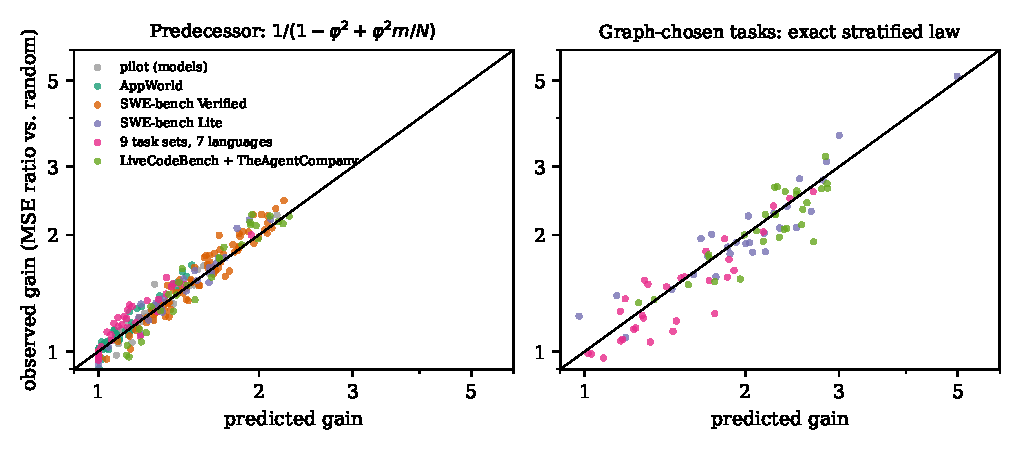
\includegraphics[width=\linewidth]{fig_law.pdf}
\caption{Predicted versus observed gain over random testing, $m=20$. Left: predecessor law (\ref{eq:law}), all six
studies (\NAll{} transitions). Right: graph law (\ref{eq:strat}) for graph-chosen tasks, studies v4--v6
(\StratN{} transitions). The diagonal is perfect prediction.}
\label{fig:law}
\end{figure}

\subsection{The graph is worth more than the predecessor}
Figure~\ref{fig:gains} summarises the gains. Using only the predecessor gives median gains of
$\times\GPredTwo$ (AppWorld), $\times\GPredThree$ (Verified), $\times\GPredFour$ (Lite), $\times\GPredFive$ (v5)
and $\times\GPredSix$ (v6). With random tasks, using the whole graph raises them in four of the five
confirmations, to $\times\GGraphTwo$, $\times\GGraphThree$, $\times\GGraphFour$ and $\times\GGraphSix$
(on SWE-bench Verified, $p=\PvalFiveVsPredThree$, paired Wilcoxon); the exception is v5 ($\times\GGraphFive$),
where most new versions solve almost nothing (Section~\ref{sec:robust}). Letting the graph also choose the tasks gives
$\times\GStratFour$ on Lite and $\times\GStratSix$ on v6, where 20 graph-chosen tasks are worth about
\EquivProbesFour{} and \EquivProbesSix{} random ones.

\begin{figure}[t]
\centering
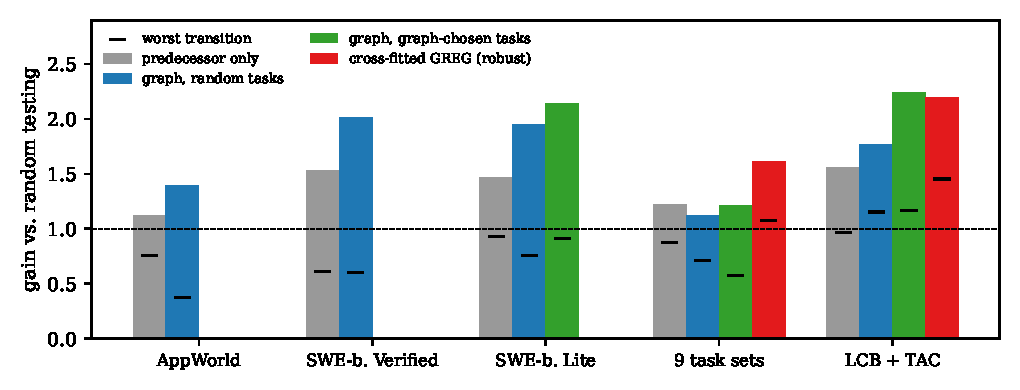
\includegraphics[width=\linewidth]{fig_gains.pdf}
\caption{Median gain over random testing ($m=20$) by study and method; black ticks mark the worst transition.
The robust estimator was introduced in v5 (its non-cross-fitted predecessor in v4 is reported in the text).}
\label{fig:gains}
\end{figure}

\paragraph{What survives a version change.} The AppWorld agents cover 14 of the 16 combinations of four scaffolds and
four models, so the type of change can be isolated (Table~\ref{tab:atlas}). A model upgrade at fixed scaffold (GPT-4 Turbo $\to$ GPT-4o)
keeps a median $\phisq=\AtlasModel$; a scaffold change at fixed model keeps \AtlasArch; a change of model family
keeps \AtlasFamily. \emph{Rewriting an agent's orchestration erases most of the transferable information---its
effect is closer to a change of model family than to a model upgrade.} When the predecessor carries nothing, the rest of the graph still does: for family changes
the graph gains $\times\AtlasGraphFamily$ where the predecessor gains $\times\AtlasPredFamily$.

\begin{table}[t]
\centering\small
\caption{Atlas of transferable information on AppWorld (v2, pre-registered, Kruskal--Wallis $p=0.0026$).}
\label{tab:atlas}
\begin{tabular}{@{}lrrrr@{}}
\toprule
Type of change & $n$ & median $\phisq$ & gain, predecessor & gain, graph\\
\midrule
Model upgrade, same scaffold & \AtlasNModel & \AtlasModel & $\times\AtlasPredModel$ & $\times\AtlasGraphModel$\\
Scaffold change, same model & \AtlasNArch & \AtlasArch & $\times\AtlasPredArch$ & $\times\AtlasGraphArch$\\
Model family change & \AtlasNFamily & \AtlasFamily & $\times\AtlasPredFamily$ & $\times\AtlasGraphFamily$\\
\bottomrule
\end{tabular}
\end{table}

\paragraph{The lineage edge is real but subsumed.} On SWE-bench Verified, a version shares more information with its
predecessor than with an unrelated earlier agent of the same success rate (median $\phisq$ \PhiLineThree{} versus
\PhiCtrlThree, pre-registered, $p<10^{-6}$). But once the difficulty seen by the whole graph is used, adding the
predecessor changes the median gain from $\times\GEcoOnlyThree$ to $\times\GGraphThreePrecise$: statistically detectable
($p=\PvalHSevenThree$) and practically negligible. The value lies in the graph, not in the lineage alone.

\subsection{Where the gain comes from (exploratory)}
The following comparisons were not pre-registered. Graph-chosen tasks are the analogue of the difficulty-stratified
subsets deployed by \citet{she2026production}; the plain mean of these tasks is therefore the natural baseline for our
estimators. That plain mean already gains $\times\GRstratFour$, $\times\GRstratFive$ and $\times\GRstratSix$ in v4,
v5 and v6. The model-based graph estimator improves on it significantly only in v4 ($p=\PStratVsRstratFour$; v6:
$p=\PStratVsRstratSix$), and GREG only in v5 ($p=\PGregVsRstratFive$; v4, without cross-fitting: $p=\PGregVsRstratFour$; v6:
$p=\PGregVsRstratSix$), where the
plain mean's worst case was $\times\GRstratMinXFive$. \emph{Most of the efficiency therefore comes from which tasks the
graph selects}---the quantity Proposition~\ref{prop:eta} predicts---while the estimator mainly buys robustness when
versions solve almost nothing, and calibration: the Clopper--Pearson intervals of the plain mean ignore the
stratification and over-cover (\CovRstratFour, \CovRstratFive, \CovRstratSix). Interval widths tell the same story. On
the development data of v5 (Lite, Verified, AppWorld), mean 90\% interval widths were \WidthReset{} for random
testing, \WidthStrat{} for the model-based graph estimator (\WidthStratRed\% narrower) and \WidthGreg{} for the
cross-fitted GREG: its intervals are calibrated, but they are not narrower than random testing's, because they stay
wide for versions with few successes.

\subsection{Robust and calibrated estimation}\label{sec:robust}
Model-based estimates can fail on versions that solve fewer than 10\% of tasks: on SWE-bench Verified the graph
estimator's worst transition was $\times\WorstVThree$ (a submission published with zero resolved tasks), while on
the \ThreeMidN{} transitions between 10\% and 90\% its worst case was $\times\ThreeMidMin$. Study v5 was dominated by
this regime (\FiveLowN{} of \NFive{} new versions below 10\%). There the cross-fitted GREG estimator gained
$\times\GGregFive$ (worst $\times\GGregMinFive$; $\times\GGregFiveLow$ below 10\%) with mean coverage \CovGregFive{}
(minimum \CovGregMinFive), whereas the model-based estimator's worst case was $\times\GStratMinFive$. In v6, where
the roles were fixed in advance, the cross-fitted estimator gained $\times\GGregSix$ (worst $\times\GGregMinSix$)
with coverage \CovGregSix{} (minimum \CovGregMinSix). The non-cross-fitted GREG of v4 never lost either (worst
$\times\GGregMinFour$) but its intervals under-covered (minimum \CovGregMinFour), which motivated cross-fitting.

\subsection{Decisions and regression detection}
On transitions where the true rates differ by at least 5 points, keep-or-replace decisions from 20 graph-chosen
tasks were wrong in \DecGraphFour\%, \DecGraphFive\% and \DecGraphSix\% of replays (v4, v5, v6), against
\DecResetFour\%, \DecResetFive\% and \DecResetSix\% with random testing (all pre-registered, $p<0.05$). In real
version histories, the sequential rule detected the \DetN{} SWE-bench Verified versions that regressed by at least
10 points in \DetPower\% of replays with \DetProbes{} probes on average, with \DetFA\% false alerts on the \DetNok{}
transitions without a drop.

\subsection{What failed}
\label{sec:failures}
Four of the \HypTotal{} pre-registered hypotheses were not supported (Appendix~\ref{app:ledger}). (i)~In the pilot,
predecessor-based estimates did not reduce decision regret significantly and (ii)~sequential detection lacked power
at 40 probes; the detection rule was retuned on development data and later confirmed in v2 and v3. (iii)~On SWE-bench
Verified the graph estimator lost badly on near-zero versions, so the hypothesis of no catastrophic loss failed. (iv)~In v5,
the model-based estimator with graph-chosen tasks did not stay above random testing on 90\% of transitions, because
most new versions solved almost nothing. Two further observations qualify our method. An unbiased estimator is not
automatically a good decision rule: in v5, GREG's decisions were wrong in \DecGregAllFive\% of replays against
\DecResetAllFive\% for random testing (\DecGregFive\% versus \DecResetFive\% on differences of at least 5 points). The
gap comes from transitions where both versions solve almost nothing: in the extreme case (both below 1\%), GREG chose
wrongly in \DecGregExtFive\% of replays and random testing in \DecResetExtFive\%, because the random baseline's
prior pushes such estimates upward and happened to point the right way. And in v6 the pre-registered decider was not the best one: the plain mean of the
graph-chosen tasks decided slightly better (\DecRstratSix\% versus \DecGraphSix\%). The robust gain in decisions comes
from \emph{which tasks are tested}; which estimator should decide remains open.

\section{The kernel: a graph of agents}
\label{sec:kernel}
The method needs a place where the graph lives. We implement it as a small kernel that observes and does not
orchestrate. State is an append-only log of events (slot and version registrations with release dates and lineage,
task results with their role and origin, probe plans); five operations act on it: \texttt{record} (one result or a
whole evaluation), \texttt{plan} (the graph chooses $m$ tasks for a new version and stores the plan, which fixes the
stratum weights), \texttt{estimate} (cross-fitted GREG on the planned probes), \texttt{decide} (keep or replace,
flagged sure or not), and \texttt{lint} (lineage inconsistencies, probes outside the plan, training tasks used as
evidence). Each slot gets a Markdown page listing its versions, estimates and intervals.

\paragraph{Validation.} Criteria fixed before the run (on data already analysed, so this tests the software, not the
method): replaying the 89 SWE-bench Verified transitions through the
kernel alone must reproduce the research gain within 10\%, keep coverage above 0.88, and make fewer decision errors
than random testing. The
kernel obtained a median gain of $\times\KernelGain$, coverage \KernelCov, and decision errors of \KernelDec\% versus
\KernelDecReset\% for random testing, with no lint finding.

\paragraph{Case study.} On the nine real OpenHands versions in SWE-bench Verified, the kernel tested 180 tasks instead
of 4{,}500. Its intervals contained the true rate for \DemoCov\% of versions and \DemoGood\% of its decisions were
right; both wrong decisions had been flagged as not sure by the kernel itself, and every decision it flagged as sure
was right.

\section{Related work}
\paragraph{Efficient evaluation.} Item response theory \citep{rasch1960} underlies tinyBenchmarks
\citep{polo2024tiny} and anchor points \citep{vivek2024anchor}, which predict benchmark scores of language models from
few items; active testing chooses test points adaptively \citep{kossen2021active}. For agents, Agent Psychometrics
predicts task-level success on coding benchmarks by separating model and scaffold abilities
\citep{ge2026psychometrics}; \citet{ndzomga2026efficient} keeps tasks with mid-range historical pass rates;
\citet{she2026production} study an evolving production agent and deploy difficulty-stratified fixed subsets with
IRT-based estimates---the closest design to our task selection, whose gain Proposition~\ref{prop:eta} predicts; \citet{johnson2026cached} estimate new agents' scores from cached traces of reference systems.
These works report point accuracy (errors, rank correlations). We add a closed-form law that predicts the gain before
testing, calibrated intervals that survive model failure, the keep-or-replace decision, and pre-registered evidence.

\paragraph{Prediction-powered inference.} PPI \citep{angelopoulos2023ppi}, PPI++ \citep{angelopoulos2023ppipp},
cross-PPI \citep{zrnic2024cross} and stratified PPI \citep{fisch2024stratified} combine model predictions with a few
labels for valid inference; \citet{mani2026nofreelunch} show that the benefit is not free in finite samples. Our
estimator is the survey-sampling counterpart (GREG with cross-fitting under a stratified design), where predictions
come from the graph of earlier agents rather than from a single predictor.

\paragraph{Version updates.} \citet{sheng2026regression} show that no single signal predicts which answers regress
after an LLM update. We do not predict individual flips; we measure how much the history reduces the cost of
estimating and deciding, which is what a team shipping a new version needs.

\section{Limitations and threats to validity}
\paragraph{Scope.} The law assumes probes drawn at random (or within strata) from a fixed task suite; it says nothing
about tasks outside the suite. Gains depend on the graph: with fewer than 20 earlier agents the median gain on SWE-bench Verified
was markedly lower. Versions that solve almost nothing remain hard for decisions. Several sources share agents or
products (SWE-bench splits; 21 of the 33 transitions in v5 are the same model change in different scaffolds and
languages), and tasks within a repository are correlated. Release dates in v6 were recorded from memory by the
research assistant (Acknowledgements). LiveCodeBench evaluates models rather than agents, and TheAgentCompany
contributes only two transitions.

\paragraph{Statistics.} Paired Wilcoxon tests treat transitions as independent units, although transitions of a study
share agents and ecosystems; their $p$-values should be read as descriptive of consistency rather than exact. The freezes are
recorded by git tags and hashes whose timestamps are self-reported, not certified by a third party; future studies
should be registered on a public registry before data access. Each study's hypotheses were tested at level 0.05 without correction across the six studies; the ledger
(Appendix~\ref{app:ledger}) reports all \HypTotal{} tests so that readers can apply their own correction. The law is
tested at the true $\rho^2$; with $\rho^2$ estimated from the probes, it was tested only in the pilot.

\paragraph{Baselines.} We compare against random testing, a predecessor-only estimator, an IRT-like logistic model on
ecosystem difficulty (v3), and the plain mean of graph-chosen tasks (exploratory). We did not re-implement
multidimensional IRT or gp-IRT \citep{polo2024tiny,she2026production}; our claims concern the law, calibration and
decisions, not point accuracy against these methods.

\paragraph{Kernel.} The kernel was validated on SWE-bench Verified, which had already been analysed; this is a test of
the software, not new evidence for the method.

\section{Conclusion}
An agent's history is worth a computable number of tasks. Across \NConf{} real version transitions in five
pre-registered confirmations, the law $1/(1-\rho^2)$ predicted that number within a few percent, and a method in which
the graph of earlier agents chooses the tasks, estimates with calibrated intervals and decides, roughly halved the cost
of evaluating a new version. Evaluation does not have to start from zero at every release: the graph of agents remembers.

\section*{Code and data availability}
Code, protocols, frozen analysis scripts with their git tags and hashes, random seeds, raw replay results and the
kernel are in the accompanying repository, which will be made public with this preprint. Every number in this paper is
generated from the result files by a script (\texttt{make\_numbers.py}). The
benchmark outputs are public: the AppWorld leaderboard bundles, the GitHub repositories
\texttt{SWE-bench/\allowbreak experiments}, \texttt{multi-swe-bench/\allowbreak experiments},
\texttt{LiveCodeBench/\allowbreak submissions} and \texttt{TheAgentCompany/\allowbreak experiments}, and the data of
\citet{sheng2026regression}.

\section*{Acknowledgements}
The author designed the study, the agent-graph framing and the research programme, and takes full responsibility
for the content. Claude (Anthropic), an AI assistant, was used extensively to write code, run the experiments and
draft the text under the author's direction; it is not an author.

\bibliographystyle{plainnat}
\bibliography{references}

\appendix
\section{Ledger of pre-registered hypotheses}
\label{app:ledger}
\begin{table}[h]
\centering\footnotesize
\begin{tabular}{@{}llp{4.2cm}p{3.6cm}@{}}
\toprule
Study & Hypothesis & Criterion (abridged) & Verdict\\
\midrule
v1 & Variability gate & $\phisq$ spread $\ge 0.20$ & supported\\
v1 & H1 law & median error $\le 0.20$ & supported (\LawErrPilot\%)\\
v1 & H2 $\phisq$ depends on pair and benchmark & Holm-corrected tests & supported\\
v1 & H3 lower decision regret & paired test & \textbf{not supported}\\
v1 & H4 regression detection & power $\ge 0.80$ & \textbf{not supported}\\
v2 & H1 law (agents) & median error $\le 0.20$ & supported (\LawErrTwo\%)\\
v2 & H5 graph $>$ predecessor & Wilcoxon, $\ge 90\%$ non-loss, coverage & supported (at the 90\% limit)\\
v2 & H2 $\phisq$ depends on type of change & Kruskal--Wallis & supported\\
v2 & H4 sequential detection & power, probes, false alerts & supported (\HFourTwoPower\%, \HFourTwoProbes{} probes)\\
v3 & H1 law & median error $\le 0.20$ & supported (\LawErrThree\%)\\
v3 & H5 graph $>$ predecessor & as v2 & supported\\
v3 & H6 no catastrophic loss & worst gain and coverage $\ge 0.80$ & \textbf{not supported}\\
v3 & H7 predecessor adds to graph & Wilcoxon & supported, negligible effect\\
v3 & H2 lineage edge carries information & Wilcoxon vs matched control & supported\\
v3 & H4 detection of real regressions & power, false alerts & supported\\
v4 & H1 law & median error $\le 0.20$ & supported (\LawErrFour\%)\\
v4 & H8 graph law & median error $\le 0.20$ & supported (\StratErrFour\%)\\
v4 & H9 graph-chosen tasks help & Wilcoxon, non-loss, coverage & supported\\
v4 & H10 better decisions & Wilcoxon & supported\\
v4 & H11 GREG no catastrophic loss & worst gain $\ge 0.80$ & supported\\
v5 & H1 law & median error $\le 0.20$ & supported (\LawErrFive\%)\\
v5 & H8 graph law & median error $\le 0.20$ & supported (\StratErrFive\%)\\
v5 & H9 graph-chosen tasks help & Wilcoxon, non-loss, coverage & \textbf{not supported}\\
v5 & H10 better decisions & Wilcoxon & supported\\
v5 & H12 robust and calibrated & worst gain, coverage & supported\\
v6 & U1 estimate: robust and calibrated & worst gain, coverage & supported\\
v6 & U2 estimate: beats predecessor-only & Wilcoxon & supported\\
v6 & U3 decide: beats random testing & Wilcoxon & supported\\
v6 & U4 both forms of the law & median errors $\le 0.20$ & supported\\
\bottomrule
\end{tabular}
\end{table}

\section{Development history}
Between studies, methods were changed only on data already analysed: the Bayesian model average of the
predecessor-only estimator (synthetic worlds, before v1); the graph estimator and the sequential rule (pilot data,
before v2); finite-population prediction, model averaging and an identifiability guard (AppWorld and pilot data,
before v3); the stratified design and GREG (SWE-bench Verified and AppWorld, before v4); cross-fitting, the
Korn--Graubard interval and the Jeffreys boundary convention (Verified, Lite, AppWorld, before v5). Variants tried and
abandoned (an empirical-Bayes slope prior; fallback rules on the number of successes) are listed in the
pre-registration documents.

\end{document}
